\documentclass{beamer}
\usepackage{amsmath,amssymb}
\usepackage{graphicx}
\usepackage{siunitx}
\sisetup{per-mode=symbol}
\usepackage{gvv}
\usepackage{listings}
\usepackage{xcolor}

% Code style
\lstset{
  basicstyle=\ttfamily\scriptsize,
  breaklines=true,
  frame=single,
  numbers=left,
  numberstyle=\tiny,
  keywordstyle=\color{blue},
  commentstyle=\color{green!50!black},
  stringstyle=\color{red!60!black},
  showstringspaces=false
}

\title{Matrix 2.10.4}
\author{ai25btech11015 -- M Sai Rithik}
\date{}

\begin{document}
\maketitle

\begin{frame}
\frametitle{Question}
Find the area of the triangle whose vertices are  
\[
A(1,-1,2), \quad B(2,0,-1), \quad C(3,-1,2),
\]  
\end{frame}

\begin{frame}
\frametitle{Vectors}
\begin{align}
\vec{A} &= \myvec{1 \\ -1 \\ 2}, \quad
\vec{B} = \myvec{2 \\ 0 \\ -1}, \quad
\vec{C} = \myvec{3 \\ -1 \\ 2} \\[1ex]
\vec{B} - \vec{A} &= \myvec{2 \\ 0 \\ -1} - \myvec{1 \\ -1 \\ 2}
= \myvec{1 \\ 1 \\ -3}, \\
\vec{C} - \vec{A} &= \myvec{3 \\ -1 \\ 2} - \myvec{1 \\ -1 \\ 2}
= \myvec{2 \\ 0 \\ 0}.
\end{align}
\end{frame}

\begin{frame}
\frametitle{Cross Product and Area}
\begin{align}
\vec{X} \times \vec{Y} &=
\myvec{
\mydet{\vec{X}_{23} & \vec{Y}_{23}} \\
\mydet{\vec{X}_{31} & \vec{Y}_{31}} \\
\mydet{\vec{X}_{12} & \vec{Y}_{12}}
} \\[1ex]
(\vec{B}-\vec{A}) \times (\vec{C}-\vec{A}) 
&= \myvec{1 \\ 1 \\ -3} \times \myvec{2 \\ 0 \\ 0}
= \myvec{0 \\ -6 \\ -2}.
\end{align}
\pause
\begin{align}
\text{Area} &= \tfrac{1}{2}\,\norm{\myvec{0 \\ -6 \\ -2}} 
= \tfrac{1}{2}\,\sqrt{0^2+(-6)^2+(-2)^2} \\
&= \tfrac{1}{2}\,\sqrt{36+4}
= \tfrac{\sqrt{40}}{2}
= \sqrt{10}.
\end{align}
\[
\boxed{\text{Area} = \sqrt{10}}
\]
\end{frame}

% ===================== FIGURE =====================
\begin{frame}
\frametitle{Figure}
\begin{center}
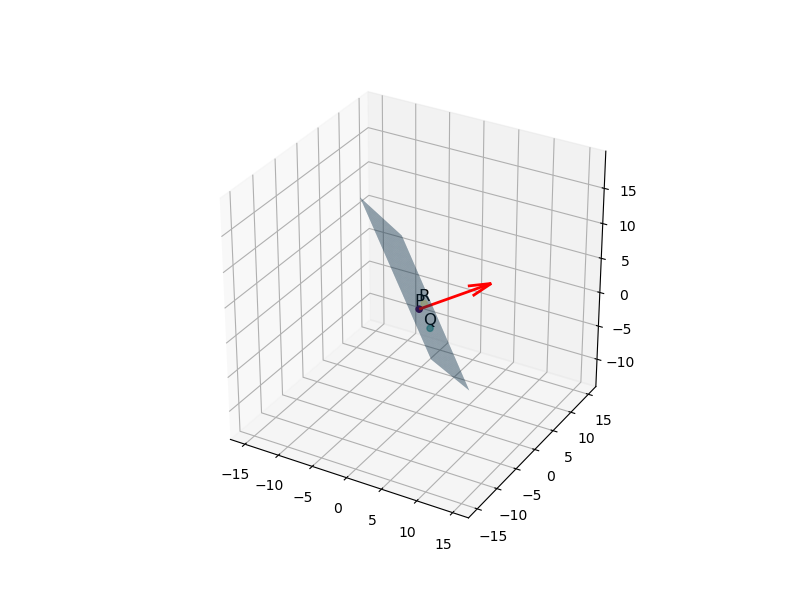
\includegraphics[width=0.7\linewidth]{figs/fig.png}
\end{center}
\end{frame}

% ===================== C CODE SLIDES =====================
\begin{frame}[fragile]
\frametitle{C Code}
\begin{lstlisting}[language=C]

#include <stdio.h>

int main() {
	int arr1[3] = {1, -1, 2};
	int arr2[3] = {2, 0, -1};
	int arr3[3] = {3, -1, 2};
	FILE *fp = fopen("var.dat", "w");
	if (fp == NULL) {
		printf("Error opening file!\n");
		return 1;
	}
	for (int i = 0; i < 3; i++) fprintf(fp, "%d%c", arr1[i], i < 2 ? ' ' : '\n');
	for (int i = 0; i < 3; i++) fprintf(fp, "%d%c", arr2[i], i < 2 ? ' ' : '\n');
	for (int i = 0; i < 3; i++) fprintf(fp, "%d%c", arr3[i], i < 2 ? ' ' : '\n');
	fclose(fp);
	return 0;
}

\end{lstlisting}
\end{frame}



% ===================== PYTHON CODE SLIDES =====================
\begin{frame}[fragile]
\frametitle{Python Code (Part 1)}
\begin{lstlisting}[language=Python]
import numpy as np
import matplotlib.pyplot as plt
from mpl_toolkits.mplot3d.art3d import Poly3DCollection
import ctypes

# #Run the C code to generate var.dat
# dll = ctypes.CDLL("./get_coordinates.so")
# dll.get_coordinates()

# Read arrays from var.dat
with open("var.dat", "r") as f:
	lines = f.readlines()
	A = np.array([int(x) for x in lines[0].split()])
	B = np.array([int(x) for x in lines[1].split()])
	C = np.array([int(x) for x in lines[2].split()])

AB = B - A
AC = C - A
# Area calculation
area = 0.5 * np.linalg.norm(np.cross(AB, AC))
print("Area of triangle ABC:", area)

# Create figure
fig = plt.figure()
ax = fig.add_subplot(111, projection='3d')

# Triangle vertices
triangle = np.array([A, B, C])
\end{lstlisting}
\end{frame}

\begin{frame}[fragile]
\frametitle{Python Code (Part 2)}
\begin{lstlisting}[language=Python]
# Plot triangle edges
ax.plot([A[0], B[0]], [A[1], B[1]], [A[2], B[2]], color='blue')
ax.plot([B[0], C[0]], [B[1], C[1]], [B[2], C[2]], color='blue')
ax.plot([C[0], A[0]], [C[1], A[1]], [C[2], A[2]], color='blue')

# Fill triangle surface
ax.add_collection3d(Poly3DCollection([triangle], color='cyan', alpha=0.5))

# Scatter vertices
ax.scatter(A[0], A[1], A[2], color='red')
ax.text(A[0], A[1], A[2], "A", fontsize=12, ha='right')
ax.scatter(B[0], B[1], B[2], color='red')
ax.text(B[0], B[1], B[2], "B", fontsize=12, ha='left')
ax.scatter(C[0], C[1], C[2], color='red')
ax.text(C[0], C[1], C[2], "C", fontsize=12, ha='center')

# Labels
ax.set_xlabel("X")
ax.set_ylabel("Y")
ax.set_zlabel("Z")
ax.set_title("Area : " + str(area))

# Save figure
plt.savefig("../figs/fig.png", dpi=300)

\end{lstlisting}
\end{frame}

\end{document}
